\section{}
\paragraph{}\label{answer:74}
مشکل این جاست که کلمات به ترتیب الفبایی در فایل ورودی ذخیره شده‌اند و درخت، نامتوازن است. بنابراین وقتی کلمات درج می‌شوند، ساختمان‌دادهٔ زیر ساخته می‌شود:
\begin{center}
    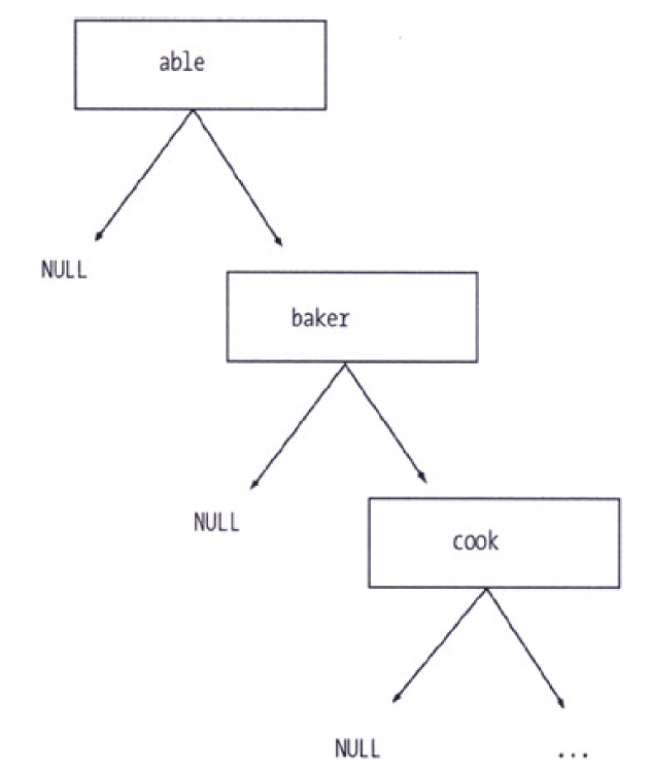
\includegraphics[keepaspectratio,width=0.4\textwidth,height=0.4\textheight]{images/image08.jpg}
\end{center}
نتیجه این است که یک لیست پیوندی داریم نه یک درخت. کلمات به انتهای لیست پیوندی اضافه می‌شوند (پرهزینه) و جستجوها به صورت خطی انجام می‌شود (باز هم پرهزینه). یک درخت متوازن می‌توانست این مشکل را حل کند.